\vspace*{-0.9cm}
\section*{I - Organisation du projet}
\addcontentsline{toc}{section}{I - Organisation du projet}
\subsection*{Méthode de travail en équipe}
\addcontentsline{toc}{subsection}{Méthode de travail en équipe}
Afin de travailler efficacement et proprement en équipe, nous avons décidé d'itérer de la façon suivante :
\begin{enumerate}
    \item \textbf{Analyse de la problématique} : avant de commencer chaque étape du projet, nous prenons le temps chacun de notre côté d'analyser et de tenter de comprendre ce qui nous est demandé.
    \item \textbf{Répartition des tâches} : nous décidons ensuite de la répartition des tâches selon les affinités de chacun et le plan que nous avons décidé de suivre.
    (Travailler chacun sur une fonctionnalité séparée, travailler ensemble sur la même fonctionnalité, \ldots)
    \item \textbf{Réalisation des tâches} : nous travaillons alors chacun sur une branche de git séparée (comme le représente la figure~\ref{fig:git_organisation}) afin de pouvoir travailler en parallèle sans se gêner.
    \item \textbf{Revue de code} : quand l'un d'entre nous a terminé une fonctionnalité, l'autre peut la fusionner sur sa branche et la tester.
    Si tout est bon, nous fusionnons sur la branche principale (master).
\end{enumerate}
Nous itérons ainsi sur les différentes fonctionnalités ou sur les corrections des possibles erreurs que nous trouvons.

\begin{figure}[h!]
    \centering
    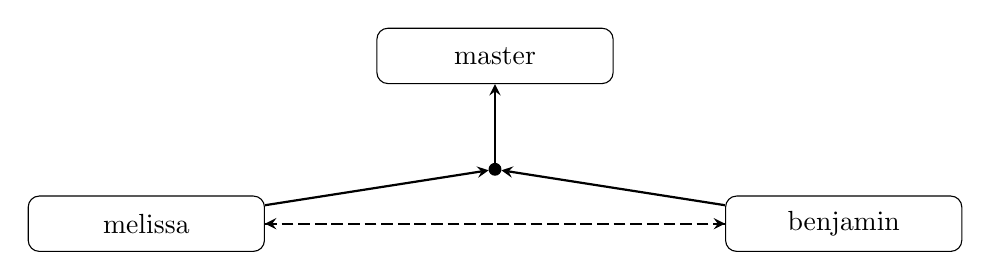
\begin{tikzpicture}[
        branch/.style={rectangle, draw, text centered, rounded corners, minimum height=2em, minimum width=3cm},
        merge/.style={circle, draw, fill=black, inner sep=1.5pt},
        main/.style={->, >=stealth, thick},
        dashedmain/.style={->, >=stealth, thick, dashed},
        node distance=2cm
    ]
    \node[branch] (master) {master};
    \node[branch, below left=of master] (melissa) {melissa};
    \node[branch, below right=of master] (benjamin) {benjamin};
    
    \node[merge, below=1cm of master] (merge1) {};
    
    \draw[main] (melissa) -- (merge1);
    \draw[main] (benjamin) -- (merge1);
    \draw[main] (merge1) -- (master);
    
    \draw[dashedmain] (melissa) -- (benjamin);
    \draw[dashedmain] (benjamin) -- (melissa);
    \end{tikzpicture}
    \caption{Organisation de nos branches de travail Git.}
    \label{fig:git_organisation}
\end{figure}

\subsection*{Organisation du code}
\addcontentsline{toc}{subsection}{Organisation du code}
Afin de rendre la navigation dans notre projet plus simple et de mieux gérer les dépendances entre les fichiers, nous avons réalisé deux fichiers par \textit{classe}\footnote{On entend par là un ensemble de fonctions, structures et variables qui sont liées entre elles par un même concept.} : un fichier \texttt{.c} qui contient les fonctions et un fichier \texttt{.h} du même nom qui contient les prototypes de ces fonctions, les structures utilisées, les variables globales et les imports.\\ \\
Chaque fichier \texttt{.h} est inclus (\texttt{\#include}) par son fichier \texttt{.c} associé, et par d'autres fichiers \texttt{.h}.
La figure~\ref{fig:file_dependencies} représente les dépendances entre chaque fichier \texttt{.h} de notre projet.\\
Ce graphique ne représente pas les fichiers de test que nous aborderons dans la section \hyperref[sec:tests]{\uline{Les tests de validation}}.\\
\begin{figure}[h!]
    \vspace*{0.3cm}
    \centering
    \usetikzlibrary{positioning}
    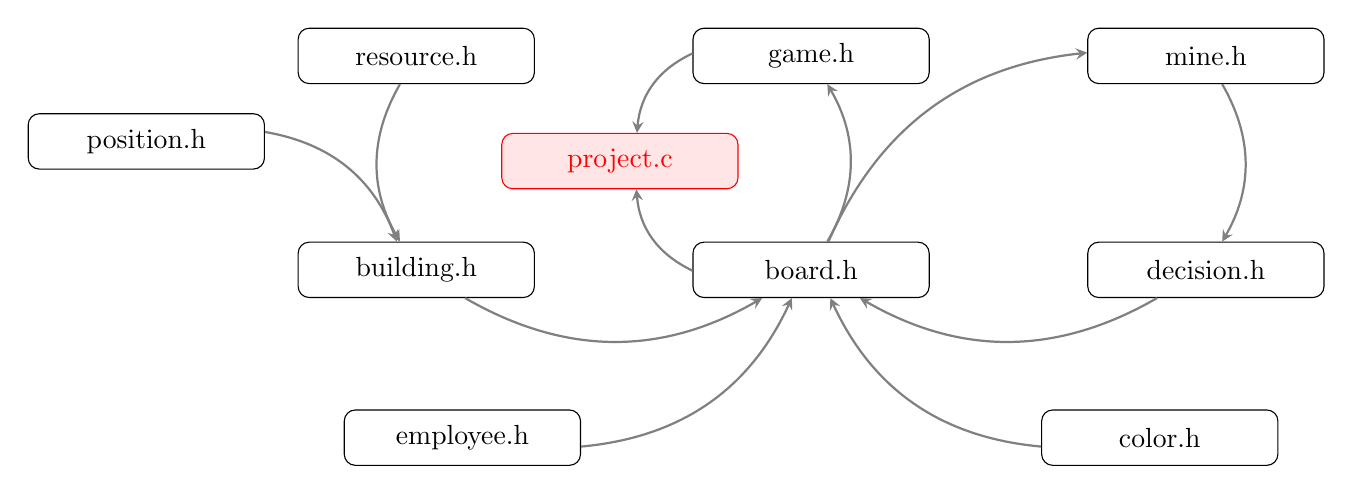
\begin{tikzpicture}[
        file/.style={rectangle, draw, text centered, rounded corners, minimum height=2em, minimum width=3cm},
            include/.style={->, >=stealth, thick},
            dashedinclude/.style={->, >=stealth, thick, dashed},
            project/.style={rectangle, draw=red, fill=red!10, text centered, rounded corners, minimum height=2em, minimum width=3cm},
            node distance=2cm
            ]
            \node[file] (game_h) {game.h};
            
        
            \node[file, below=of game_h] (board_h) {board.h};
            \node[file, right=of board_h] (decision_h) {decision.h};
            \node[file, left=of board_h] (building_h) {building.h};
            \node[file, above=of decision_h] (mine_h) {mine.h};
           
            \node[file, above left=of building_h, xshift=1cm, yshift=-0.5cm] (position_h) {position.h};
            \node[file, above=of building_h] (resource_h) {resource.h};
            \node[file, below right=of board_h] (color_h) {color.h};
            
            \node[project, above left=of board_h, text=red, xshift=2cm, yshift=-0.75cm] (project_c) {project.c};
            \node[file, below left=of board_h] (employee_h) {employee.h};
            
            \draw[include, gray, bend left] (position_h) to (building_h);

    \draw[include, gray, bend right] (game_h) to (project_c);

    \draw[include, gray, bend left] (board_h) to (project_c);
    \draw[include, gray, bend right] (employee_h) to (board_h);
    \draw[include, gray, bend right] (building_h) to (board_h);
    \draw[include, gray, bend right] (resource_h) to (building_h);
    \draw[include, gray, bend left] (color_h) to (board_h);
    \draw[include, gray, bend left] (mine_h) to (decision_h);
    \draw[include, gray, bend left] (decision_h) to (board_h);
    \draw[include, gray, bend left] (board_h) to (mine_h);

    \draw[include, gray, bend right] (board_h) to (game_h);
    \end{tikzpicture}
    \caption{Dépendances entre les fichiers du projet basées sur les inclusions. Les flèches pointent des fichiers inclus vers les fichiers qui les importent.}
    \label{fig:file_dependencies}
\end{figure}
\noindent Celui-ci nous permet de visualiser que le fichier \texttt{board} est le fichier central de notre projet, il inclut la plupart des autres fichiers et permet avec \texttt{game} de compléter la fonction d'exécution principale.\\
Cependant, on observe de possibles améliorations avec des dépendances cycliques entre les fichiers \texttt{decision}, \texttt{board} et \texttt{mine}, ainsi que \texttt{project}, \texttt{game} et \texttt{board}.\\
Pour rendre notre projet plus facile à exécuter, nous avons mis en place un \texttt{Makefile} afin de compiler l'ensemble de nos fichiers sources en un seul exécutable, mais aussi de pouvoir compiler et exécuter les tests aisément (voir section \hyperref[sec:tests]{\uline{Les tests de validation}}).\\
Celui-ci est composé de telle sorte à ce que chaque nouveau fichier .c dans le dossier \texttt{src/} soit automatiquement ajouté à la compilation de l'exécutable principal, de même pour les tests. \\
Ainsi, la commande \texttt{make} permet de compiler l'ensemble du projet et la commande \texttt{make test} permet de lancer les tests.

\subsection*{Les tests de validation}
\addcontentsline{toc}{subsection}{Les tests de validation}
\label{sec:tests}
Afin de s'assurer que chaque fonction de notre projet fonctionne correctement tout au long du développement de celui-ci, nous avons mis en place des tests unitaires.\\ \\
\begin{minipage}{0.4\textwidth}
    \begin{figure}[H]
        \centering
        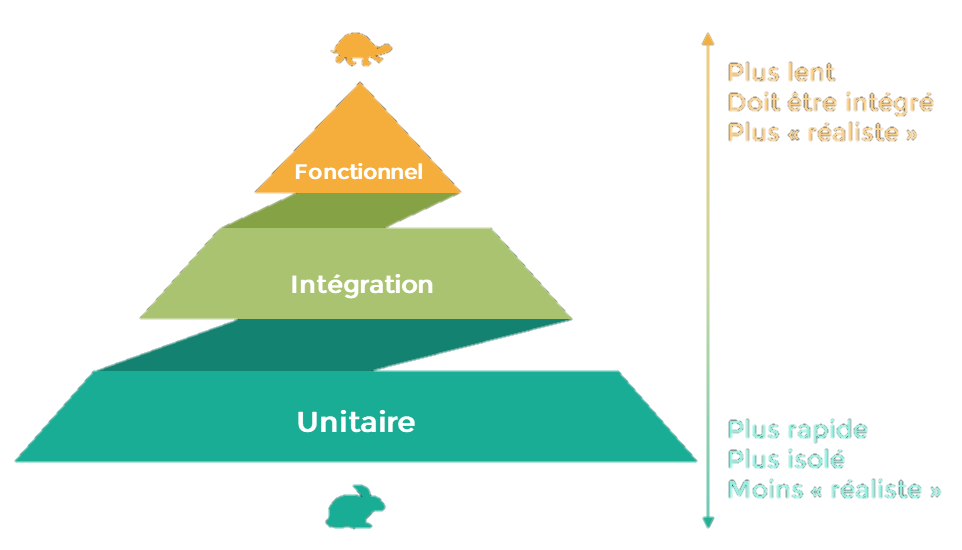
\includegraphics[width=\textwidth]{img/tests.png}
        \caption{Pyramide des tests~\cite{openclassrooms_pyramide_tests}}
        \label{fig:test_pyramid}
    \end{figure}
\end{minipage}\hfill
\begin{minipage}{0.55\textwidth}
Il existe différents types de tests, la figure~\ref{fig:test_pyramid} représente les principaux.
Mais nous avons choisi de réaliser uniquement des tests unitaires pour ce projet, car plus simples et plus rapides à mettre en place, ils semblaient suffisants pour vérifier le fonctionnement de notre projet.\\ \\
Plusieurs librairies \texttt{C} permettent de réaliser des tests unitaires telles que \texttt{cmocka} \cite{cmocka2025}.
Dans le contexte de ce projet, nous n'avons pas utilisé de librairies pour mieux comprendre ce que nous manipulions.\\
\end{minipage}
Pour tester nos fonctions unitairement, nous avons réalisé un fichier de test par fichier source de notre projet, contenant chacun des fonctions de tests pour les fonctions essentielles de celui-ci.\\
Un fichier général \texttt{test.c} permet de lancer l'ensemble des tests de notre projet.
